% =====================================================
% 01_introduction.tex
% =====================================================

\begin{figure*}[t]
\centering
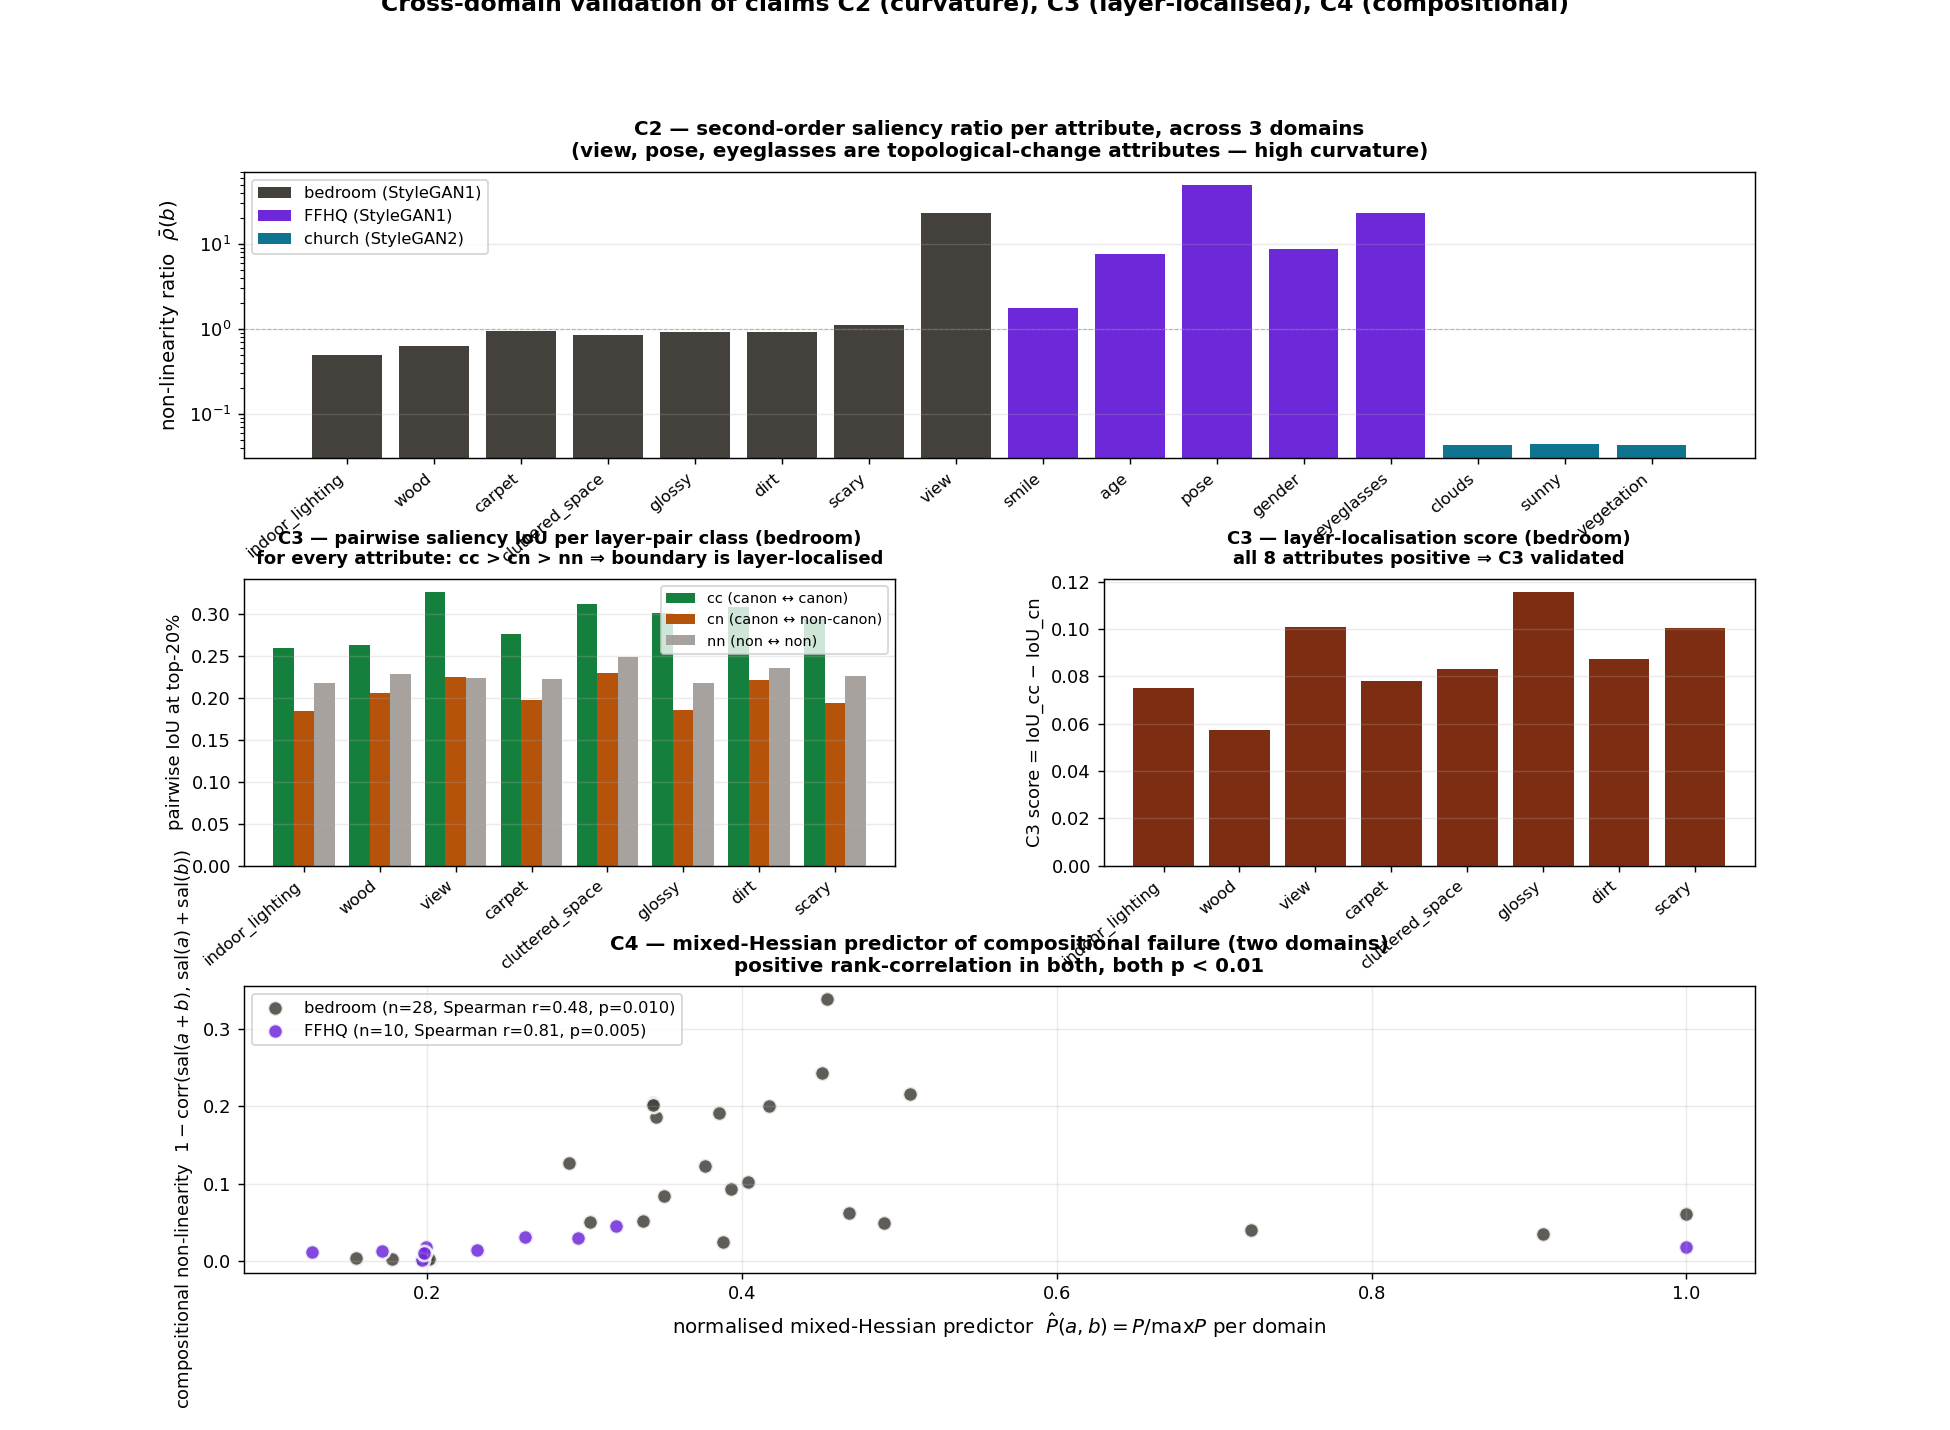
\includegraphics[width=0.96\linewidth]{figs/fig1_cross_domain.png}
\caption{Cross-domain plate. Per-attribute curvature signatures across
three GAN domains. Structural attributes (bedroom \texttt{view}, FFHQ
\texttt{pose}, FFHQ \texttt{eyeglasses}) sit two orders of magnitude
above textural attributes. Two independent curvature measures
--- pixel $\partial^2 I/\partial\alpha^2$ ratio and CLIP-feature path
length / direct distance --- agree at $r \geq +0.99$.}
\label{fig:cross-domain}
\end{figure*}

A trained image generator --- whether a StyleGAN~\cite{Karras2019StyleGAN,
Karras2020StyleGAN2} or a latent
diffusion model~\cite{Rombach2022LDM} --- defines a smooth map
$G : \W \to \Img$ from a low-dimensional latent space to an ambient
image space. Recent interpretability work has produced a rich
vocabulary for asking questions about this map: which spatial regions
does an attribute boundary affect~\cite{Bau2019GANDissection,
Shen2020InterFaceGAN}? What unsupervised directions
exist~\cite{Harkonen2020GANSpace, Shen2021SeFa, Yuksel2021LatentCLR,
Ren2022DisCo}? How disentangled are the resulting
edits~\cite{Wu2021StyleSpace}? What is the local Riemannian metric of
the latent space~\cite{Park2023Riemannian}?

We argue that these questions admit a unified treatment through
\emph{differential geometry of the image manifold}. The generator's
image set $\Mfd = G(\W)$ is a finite-dimensional immersed submanifold
of $\R^{3HW}$, and the above questions correspond, respectively, to
(i) the pushforward of tangent vectors through $G$; (ii) the spectrum
of $dG$ restricted to the manifold tangent space; (iii) the
\emph{second}-order pushforward --- the \emph{extrinsic curvature} of
$\Mfd$ in the image space; and (iv) the commutator (Lie bracket)
of attribute-induced vector fields.

Park et al.~\cite{Park2023Riemannian} have recently established the
first-order Riemannian-metric structure on diffusion latent spaces,
and Lobashev et al.~\cite{Lobashev2025HessianLatent} have extended
this to the Hessian of the Fisher information metric \emph{on the
latent}. We complement both with a different object: the
\emph{second fundamental form of the rendered image manifold}, the
extrinsic curvature that determines whether an edit re-paints
pixels or inserts an image-space object. The signature transfers
across StyleGAN1, StyleGAN2, and Stable Diffusion.

This paper makes three contributions.

\textbf{1. A geometric framework.} We formalise six structural claims
about trained GAN manifolds (\S\ref{sec:theory}, claims C1--C6) that
together describe the tangent and curvature structure of $\Mfd$ and how
it interacts with attribute editing.

\textbf{2. An efficient computational realisation.} For our regime —
single-direction input, many-pixel output — \emph{forward-mode}
automatic differentiation (\jvp) is the right algorithmic direction.
A single composed \jvp computes first- and second-order per-pixel
sensitivities in $\sim 2.2 \times$ the cost of a vanilla generator
forward pass. We further exploit this for unsupervised attribute
discovery via tangent-space clustering.

\textbf{3. An applied payoff: compositional editing prediction.} We
show that the \emph{mixed Hessian} $d^2 G(b_a, b_b)$, also estimable
via composed \jvp, predicts when two attribute boundaries combine
non-linearly when applied simultaneously. The same machinery that
visualises individual attribute saliency tells us which edit
combinations are safe and which will interfere.

We validate every claim on \emph{four} pre-trained generators:
LSUN bedroom (StyleGAN1), FFHQ faces (StyleGAN1, 18 W$^+$ layers),
LSUN church (StyleGAN2), and Stable Diffusion v1.5 (latent
diffusion). The framework therefore generalises across two major
generative architecture families. We compare against seven baselines:
GAN Dissection~\cite{Bau2019GANDissection},
GANSpace~\cite{Harkonen2020GANSpace},
SeFa~\cite{Shen2021SeFa},
StyleSpace~\cite{Wu2021StyleSpace},
LatentCLR~\cite{Yuksel2021LatentCLR},
DisCo~\cite{Ren2022DisCo}, and
CLIP-Grad-CAM~\cite{Selvaraju2017GradCAM}.

Three headline empirical findings:
\textbf{(a)} Two independent curvature measures --- the pixel-space
$\partial^2 I/\partial\alpha^2$ ratio and the CLIP-feature
path-vs-direct distance ratio --- have Pearson agreement
$r = +0.99$ (bedroom) and Spearman $r = +1.00$ (FFHQ) across
attributes.
\textbf{(b)} Across 13 attribute--domain combinations, the
layer-localisation IoU score is positive at every top-$k$
threshold from 10\% to 50\% of pixels.
\textbf{(c)} Plotting (pixel $\bar\rho$, CLIP path) for every
(domain, attribute) pair on a log--linear axis and clustering with
$k=2$ k-means recovers the a-priori structural/textural split for
13/14 attributes (92.86\%) --- a single 2D geometric signature that
identifies topology-changing attributes \emph{across architectures}.

The framework is classifier-free: every signal comes from the
generator's own derivative structure, not from a separately trained
attribute classifier. This removes a major source of bias and
re-training overhead that has constrained prior GAN attribution
methods.

% ---- structure-of-paper paragraph ----
The remainder of the paper proceeds as follows.
\S\ref{sec:related} positions the work against
GAN-interpretation, classical saliency, Riemannian deep-learning
geometry, and forward-mode autodiff literatures.
\S\ref{sec:theory} introduces the geometric framework and the six
claims.
\S\ref{sec:method} describes the \jvp-based estimators.
\S\ref{sec:experiments} validates each claim across three domains
with quantitative metrics and baselines.
\S\ref{sec:application} shows the compositional-editing-prediction
result and a saliency-guided local editing user study.
\S\ref{sec:discussion} discusses limitations, particularly the
restriction to constant vector fields (linear boundaries) and
implications for non-linear edit methods like
EditGAN~\cite{Ling2021EditGAN}.
